\s{超流動転移温度に対する不純物効果}\label{sec:bcsl:con}

\begin{figure}[t]
\centering
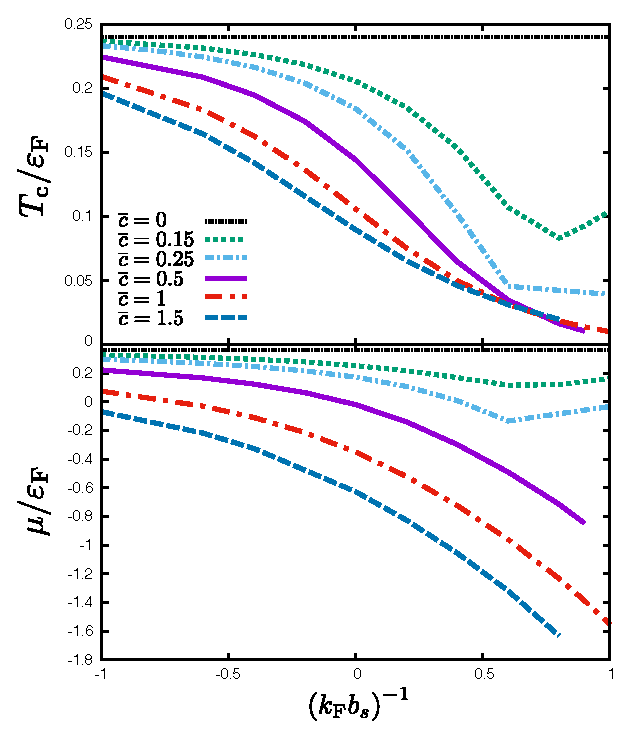
\includegraphics[width=90mm]{eps/tma-cpt-all.eps}
\caption{ユニタリー極限 $\askfi=0$ における (a) 超流動転移温度 $\tc$ と (b)  化学ポテンシャル $\cpt (\tc)$ 。}
\label{fig:bcsl:con:tma-all}
\end{figure}



\begin{figure}[t]
\centering
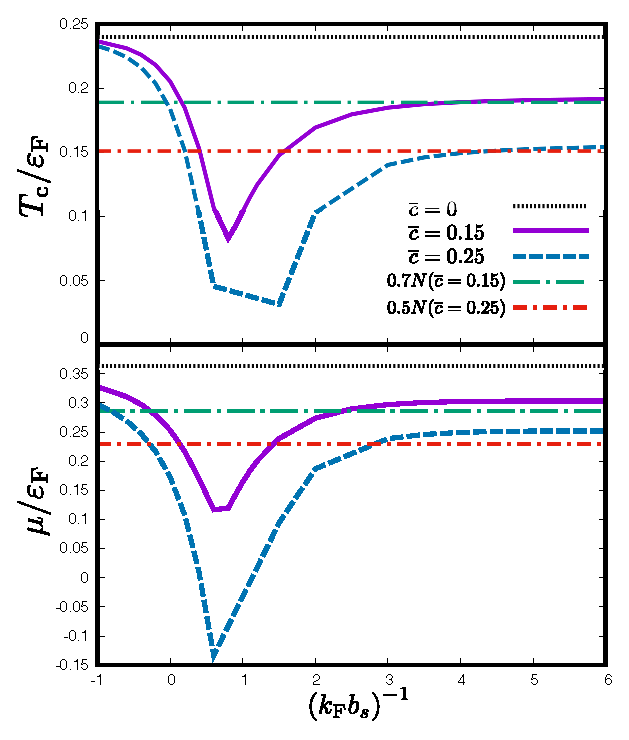
\includegraphics[width=90mm]{eps/tma-cpt-large.eps}
\caption{ユニタリー極限 $\askfi=0$ における (a) 超流動転移温度 $\tc$ と (b) 化学ポテンシャル $\cpt(\tc)$ の不純物濃度 $\overline{c}=0.15,\ 0.25$ について不純物散乱強度依存性をプロットしている。また $(1-2\lc)N$ 粒子の純粋系における値も図中に示した。}
\label{fig:bcsl:con:tma-wide}
\end{figure}

\begin{figure}[t]
\centering
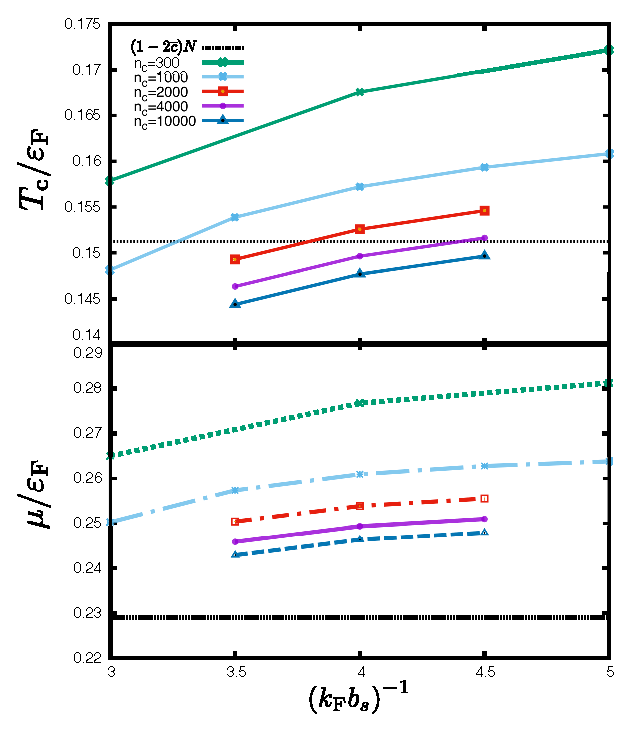
\includegraphics[width=90mm]{eps/tma-cpt-cut.eps}
\caption{ユニタリー極限 $\askfi=0$ における超流動転移温度 $\tc$ と (b) 化学ポテンシャル $\cpt(\tc)$ のフェルミオンの松原周波数のカットオフ $n_{\text{c}}$ 依存性。$(1-2\lc)N$ 粒子の純粋系における値も図中に示した。}
\label{fig:bcsl:con:tma-cut}
\end{figure}



図 \ref{fig:bcsl:con:tma-all} はユニタリ極限における超流動転移温度 $\tc$、および、化学ポテンシャル $\cpt$ に対する不純物散乱強度依存性である。この結果は、\ref{sec:form:tmat} 節の式 (\ref{eq:form:ham:sctma}), (\ref{eq:form:tma:gimp}), (\ref{eq:form:tma:gall})-(\ref{eq:form:tma:piimp}) を自己無撞着に解いて得られたものである。

不純物濃度 $\lc=0.5$ の場合、$T=0$ では$\bskfi=1.1$ で、超流動が消失 $\del=0$ したが、それを反映し、$\tc$ も $\bskfi=1$ に近づくと急速に減少する。今の計算では松原周波数の和を取るため、完全に $T=0$ とする計算はできず、$\lc=0.5$ での $\tc$ が完全に 0 になるところまでは数値的に確認できないが、 $\bskfi\gg1$ では全フェルミ原子が不純物に束縛されることを考慮すると、最終的には $\bskfi\sim1$ で$T_{\text{c}}=0$ となることが予想される。

不純物濃度が $\lc=1.0,\ 1.5\  (>0.5)$ の場合にも、$\bskfi\gtsim 0$ では $\tc$ は急速に減少するが、$\bskfi \sim 1$ で $\lc=0.5$ よりも高い $\tc$ を取るようになる。後に議論するカットオフ依存性に関係し、高い $\tc$ をとる $\bskfi$ の値は大きくなりうるが、この時は不純物バンドは“伝導バンド”から完全に分離しても部分的に占有されるだけなので $\lc=0.5$ の時と異なり $\bskfi$ が大きい領域でも $\tc$ は有限に残る。

$\lc <0.5$ の場合、$T=0$ での議論から $\bskfi \gg 1$ でも不純物に束縛されなかった $N'=N(1-2\lc)$ のフェルミ原子が超流動転移を起こすと考えられるので、$\tc>0$ となるはずである。実際 $\lc=0.15,\ 0.25$ の場合、不純物散乱強度を強くすると、$\bskfi\sim1$ で一旦は $\tc$ は減少するものの、$\bskfi\gg1$ では予想どおり一定値に近づいていく。

$\bskfi \gg 1 $ では不純物に束縛されなかった $N'=N(1-2\lc)$ 個の原子による超流動と考えられるので、この極限では不純物がない場合の$\tc$ を$\tc^{0}$ とすると、
\beq
T_c=\left(1-2 \lc\right)^{\frac{2}{3}} T_c^0,\label{eq:bcsl:con:tctc0}
\eeq
と評価できる。同様に化学ポテンシャルも不純物がない場合の値 $\cpt^0$ を用い、
\beq
\cpt=\left(1-2 \lc\right)^{\frac{2}{3}} \cpt^0,\label{eq:bcsl:con:cpcp0}
\eeq
と評価される。


図 \ref{fig:bcsl:con:tma-wide} では、$\bskfi\gg1$ での $\tc$ や $\cpt(\tc)$ は完全には式 (\ref{eq:bcsl:con:tctc0}), (\ref{eq:bcsl:con:cpcp0}) に一致していないが、これは今の数値計算が松原周波数の無限の和を有限なところで打ち切っていることに因る。すなわち、数値計算で、粒子数を本研究では、
\beq
N = 2T \sum_{\bp}\sum_{n=-n_{\rm c}}^{n_{\rm c}} \gpom e^{i \omn \delta},
\eeq
と計算している。図 \ref{fig:bcsl:con:tma-wide} では $n_{\rm c}=4000$ としているが、この $n_{\rm c}$ を変えると、より大きな $n_{\rm c}$ まで和を取ると $\tc$ は次第に式 (\ref{eq:bcsl:con:tctc0}) に $\bskfi\gg1$ で近づいていくことが見て取れる(図 \ref{fig:bcsl:con:tma-cut})。一方で、式 (\ref{eq:bcsl:con:cpcp0}) へは完全には近づかないが、これは不純物による定数的な化学ポテンシャルシフトが入っているためである。このことは次に示す、$\bskfi \simeq 3$ における状態密度がクリーン系の $N'=(1-2\lc)N$ の状態密度に漸近することから確認できる。以下では $n_{\rm c}=4000$ とする。

\begin{figure}[t]
\centering
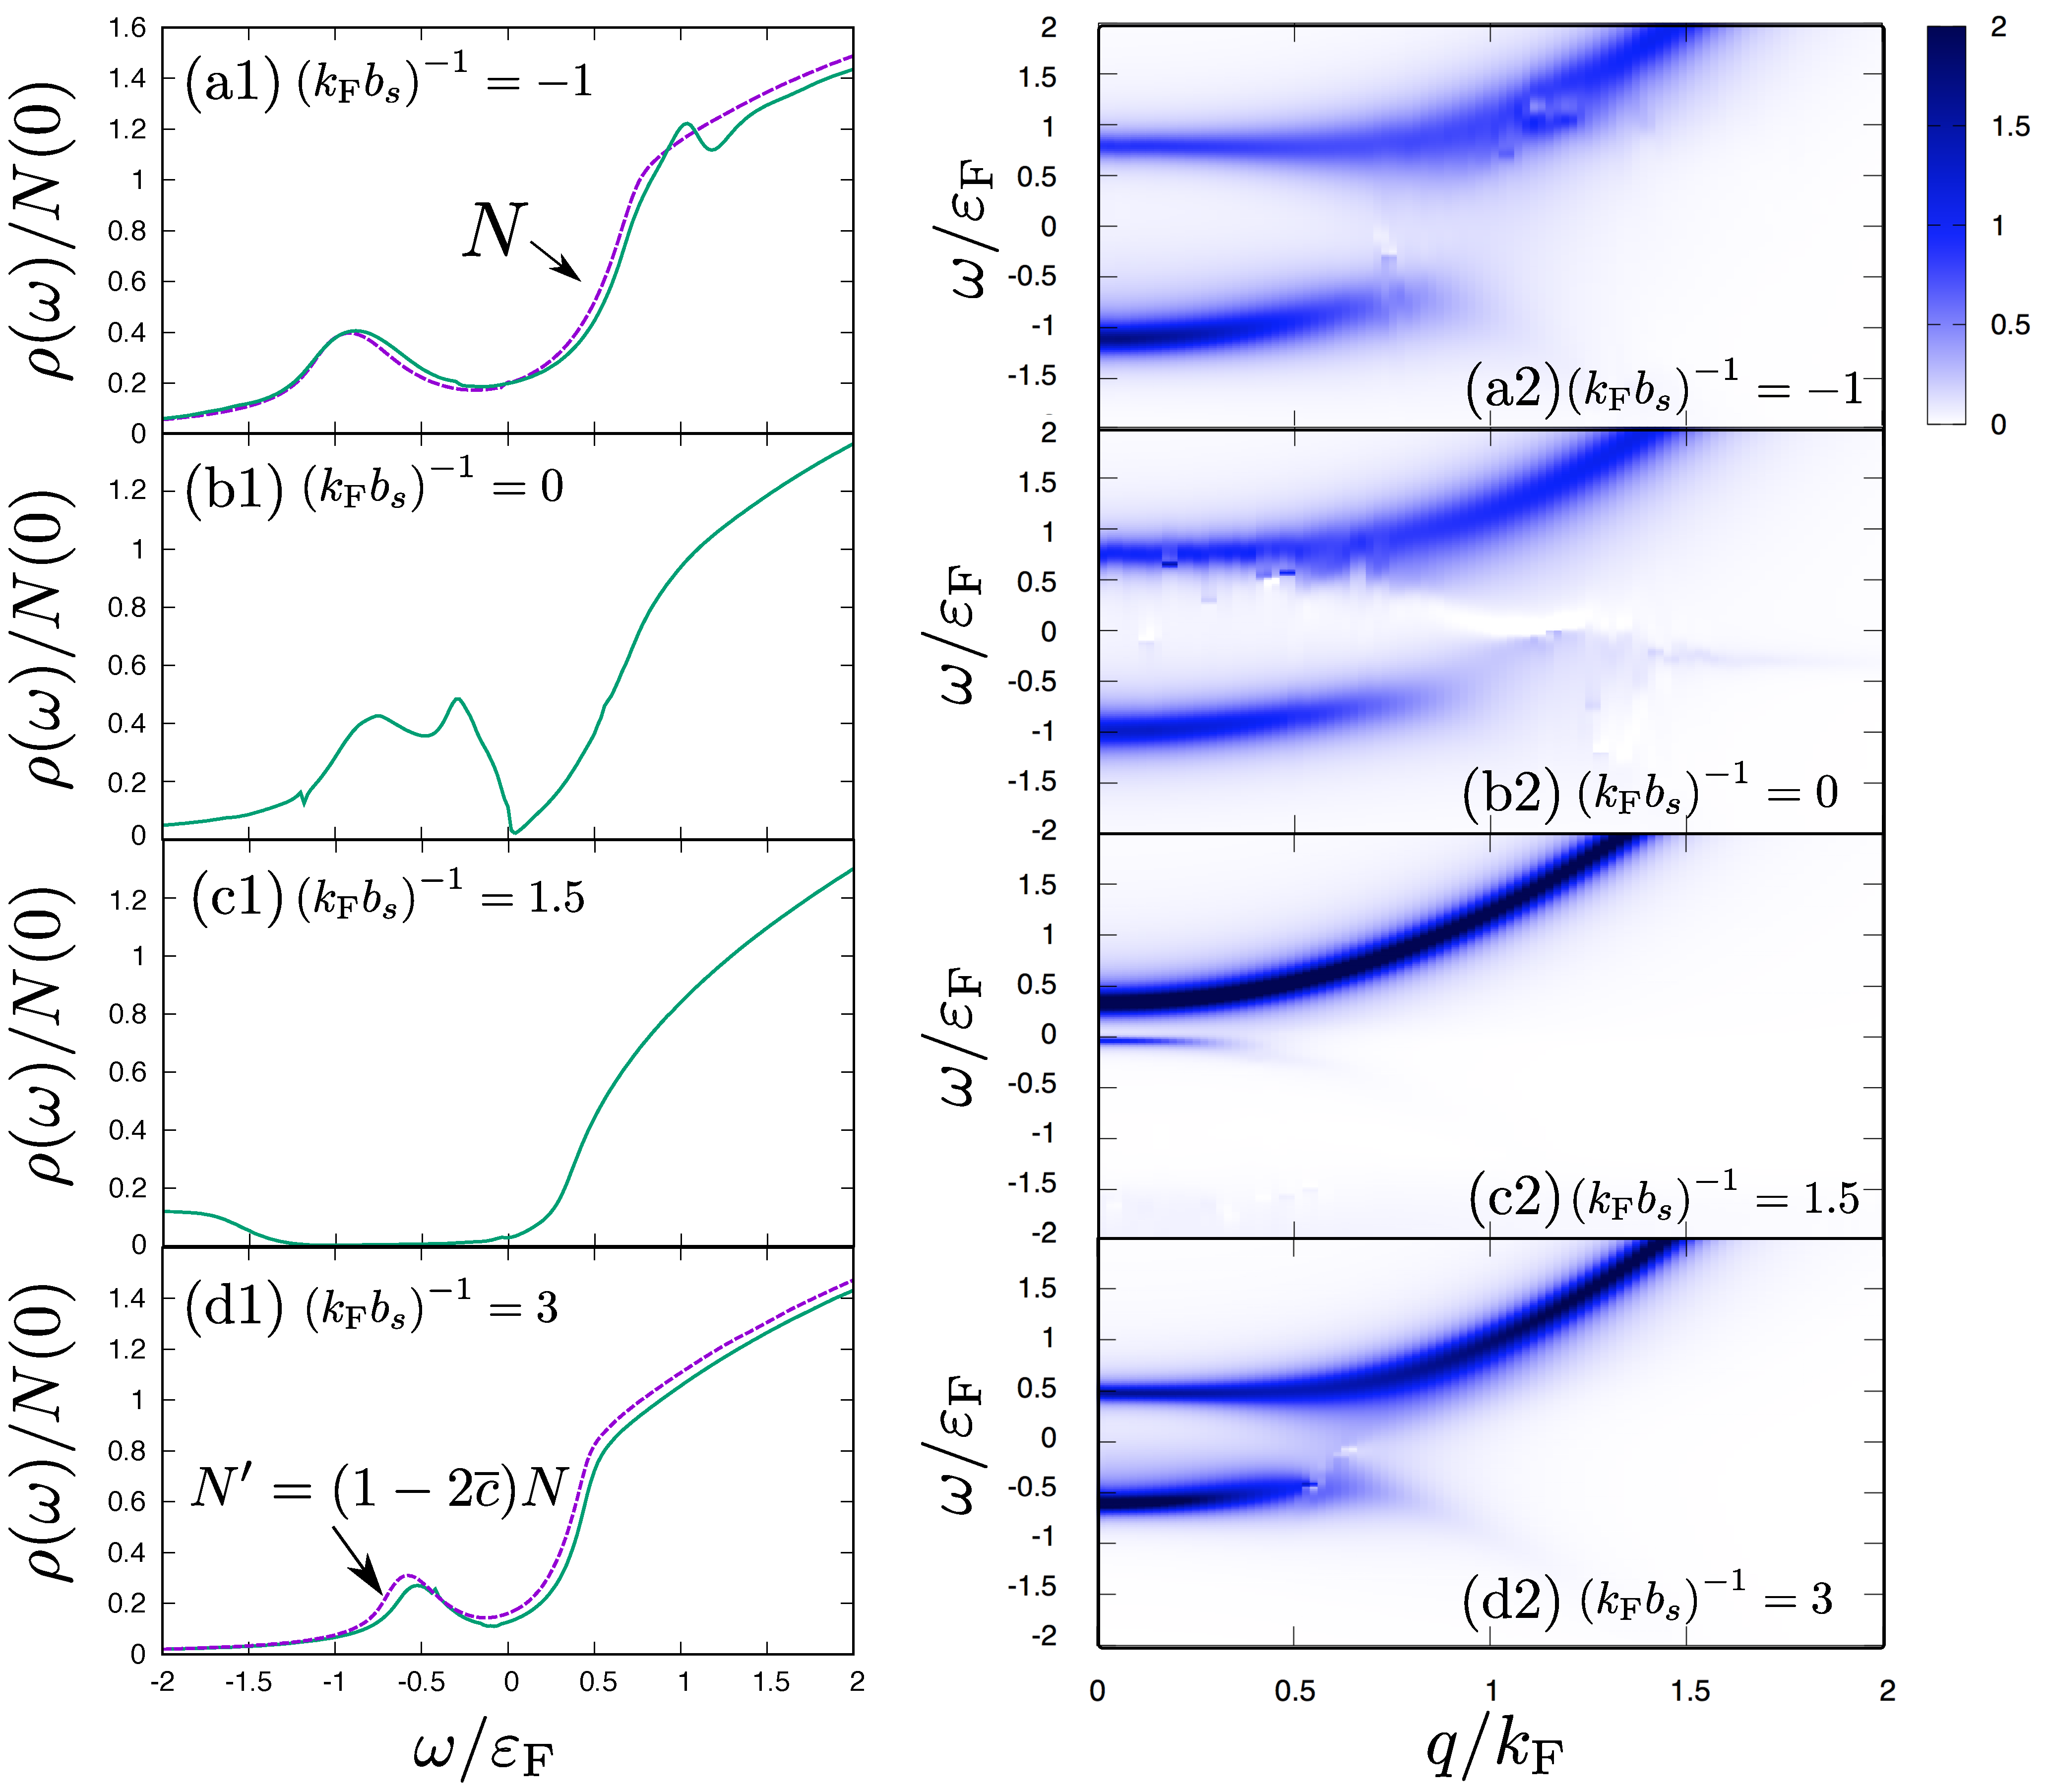
\includegraphics[width=130mm]{eps/tma-c0250-spe.eps}
\caption{$\overline{c}=0.25$、$T=\tc$ における 1 粒子状態密度(左)とスペクトル強度(右)。原子間引力相互作用はユニタリ極限 $\askfi=0$ にとってある。(a1) の破線は $N$ 粒子のクリーン系、(d1) の破線は $N'=(1-2\lc)N$ 粒子のクリーン系における擬ギャップ構造を有する状態密度。}
\label{fig:bcsl:imp:psgap}
\end{figure}

\begin{figure}[t]
\centering
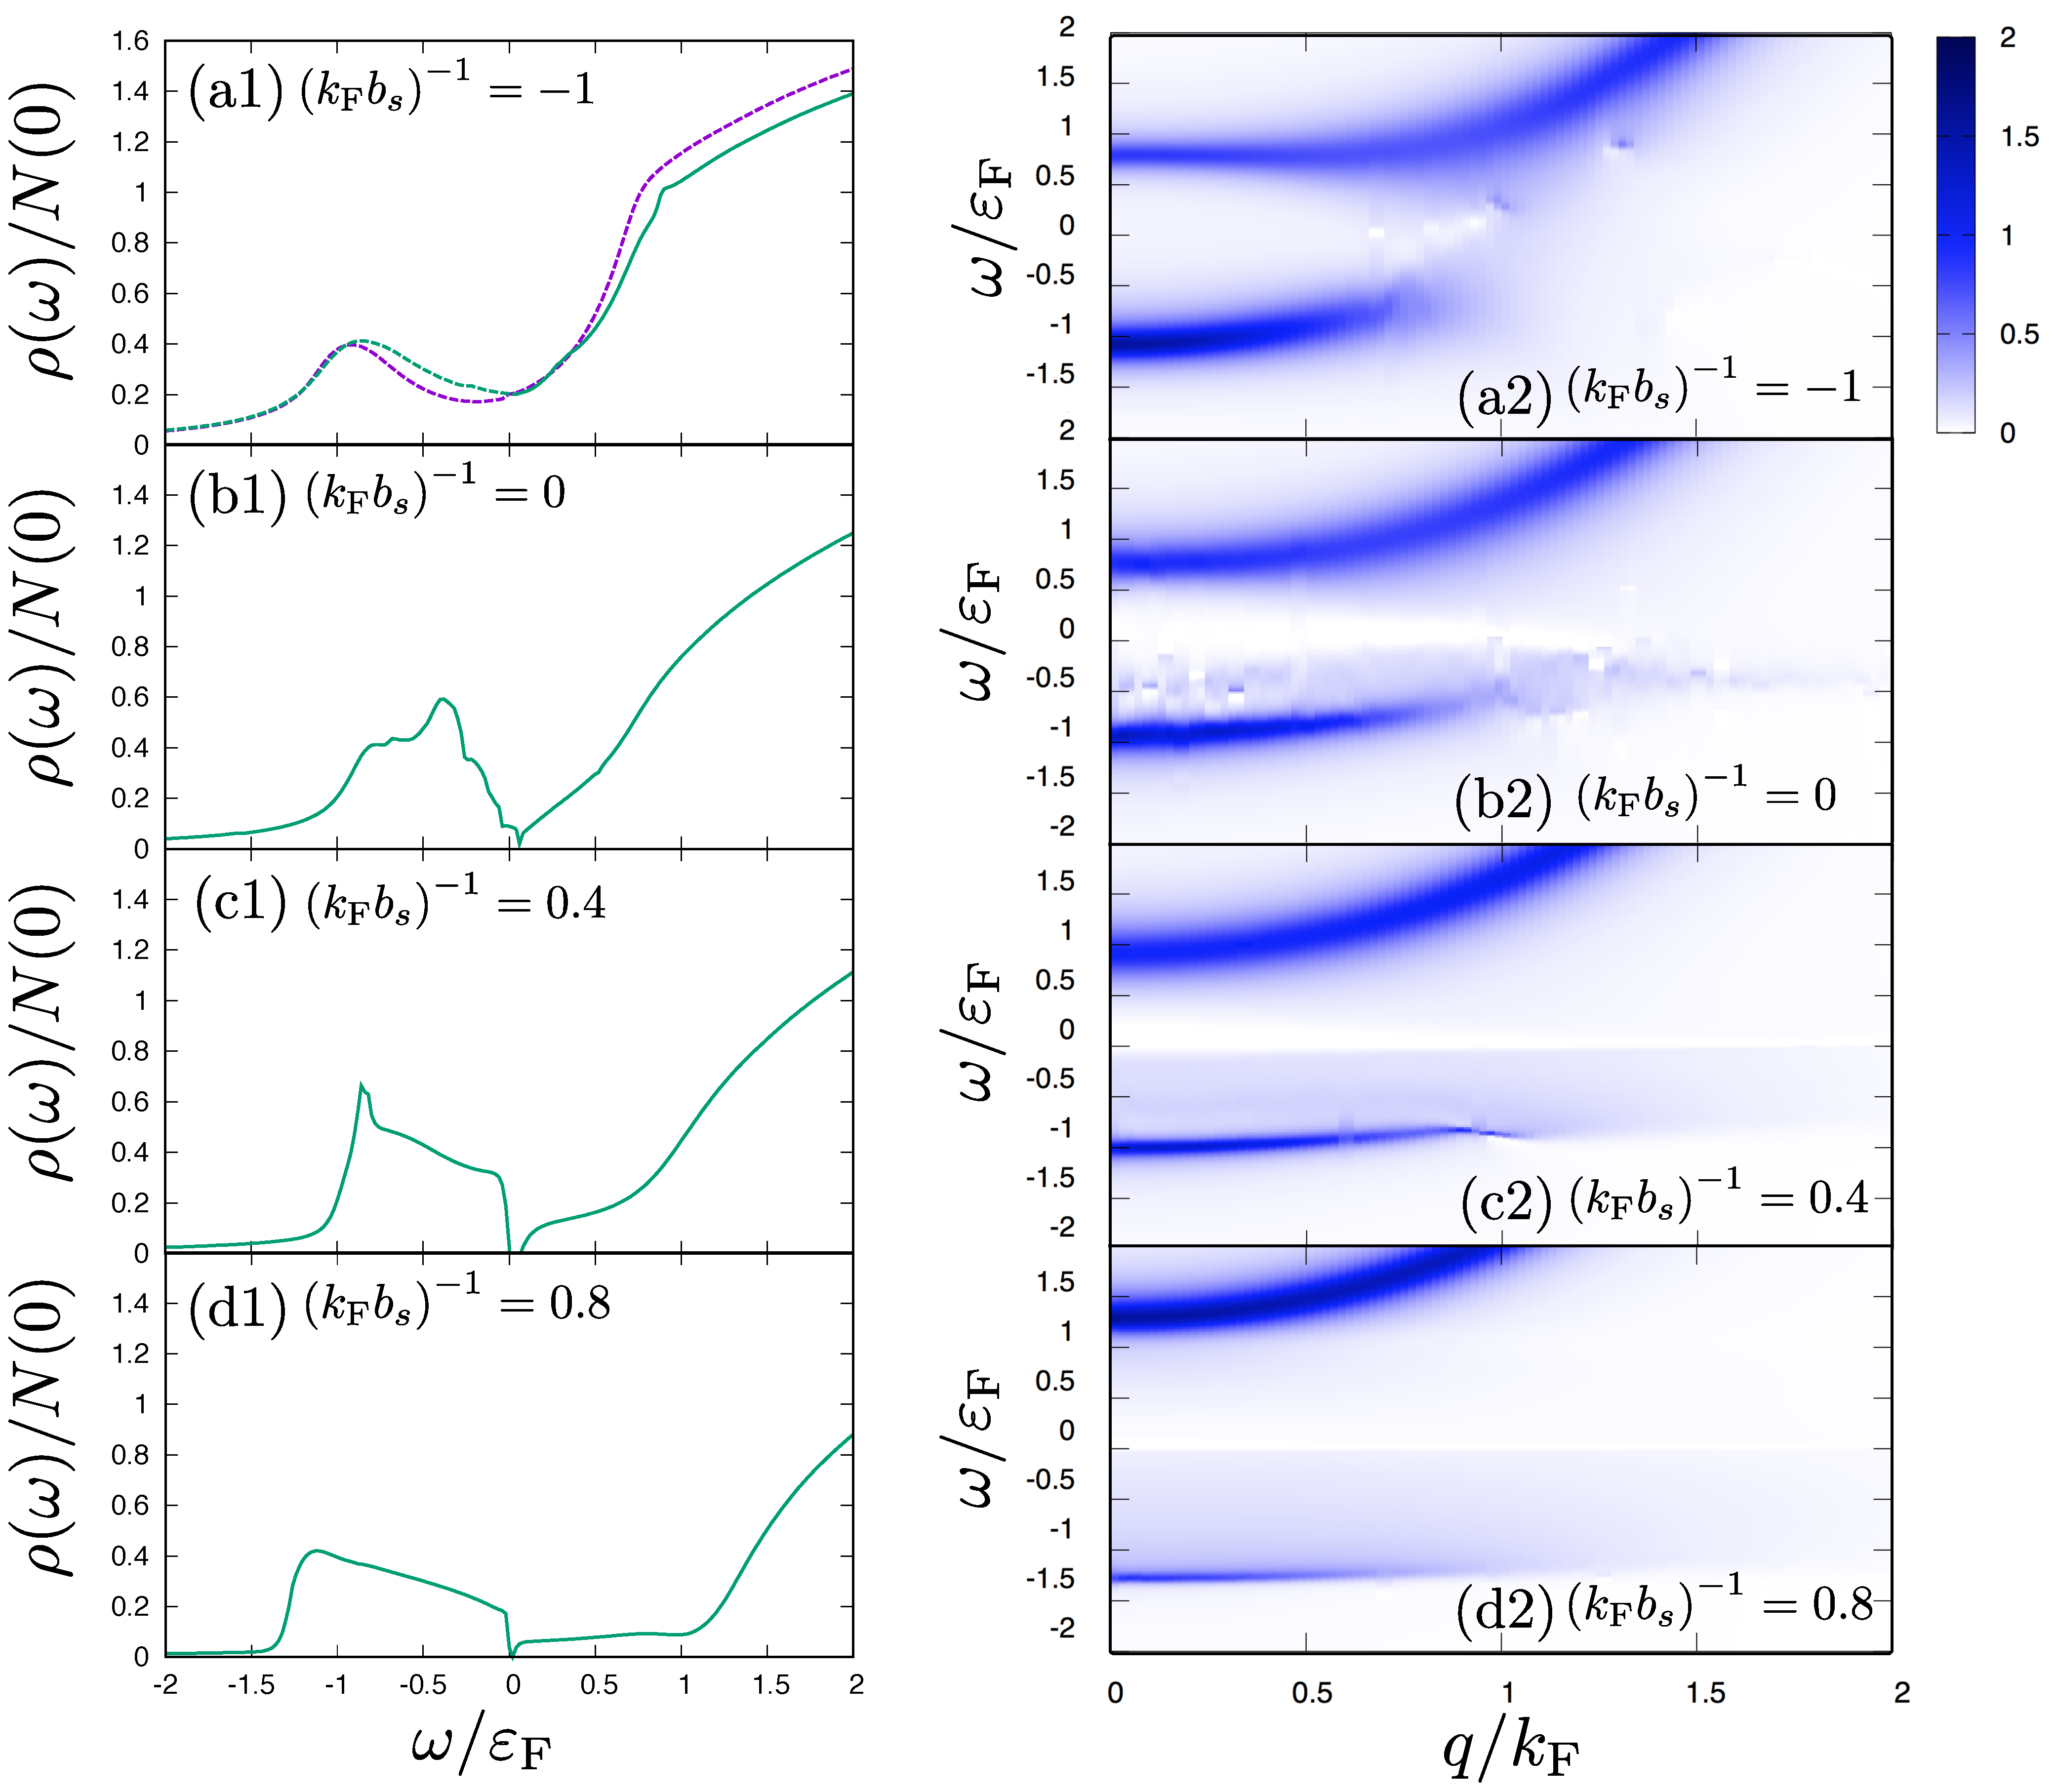
\includegraphics[width=130mm]{eps/tma-c0500-spe.eps}
\caption{図 \ref{fig:bcsl:imp:psgap} と同じだが $\overline{c}=0.5$ の場合。}
\label{fig:bcsl:imp:psgap1}
\end{figure}

\begin{figure}[t]
\centering
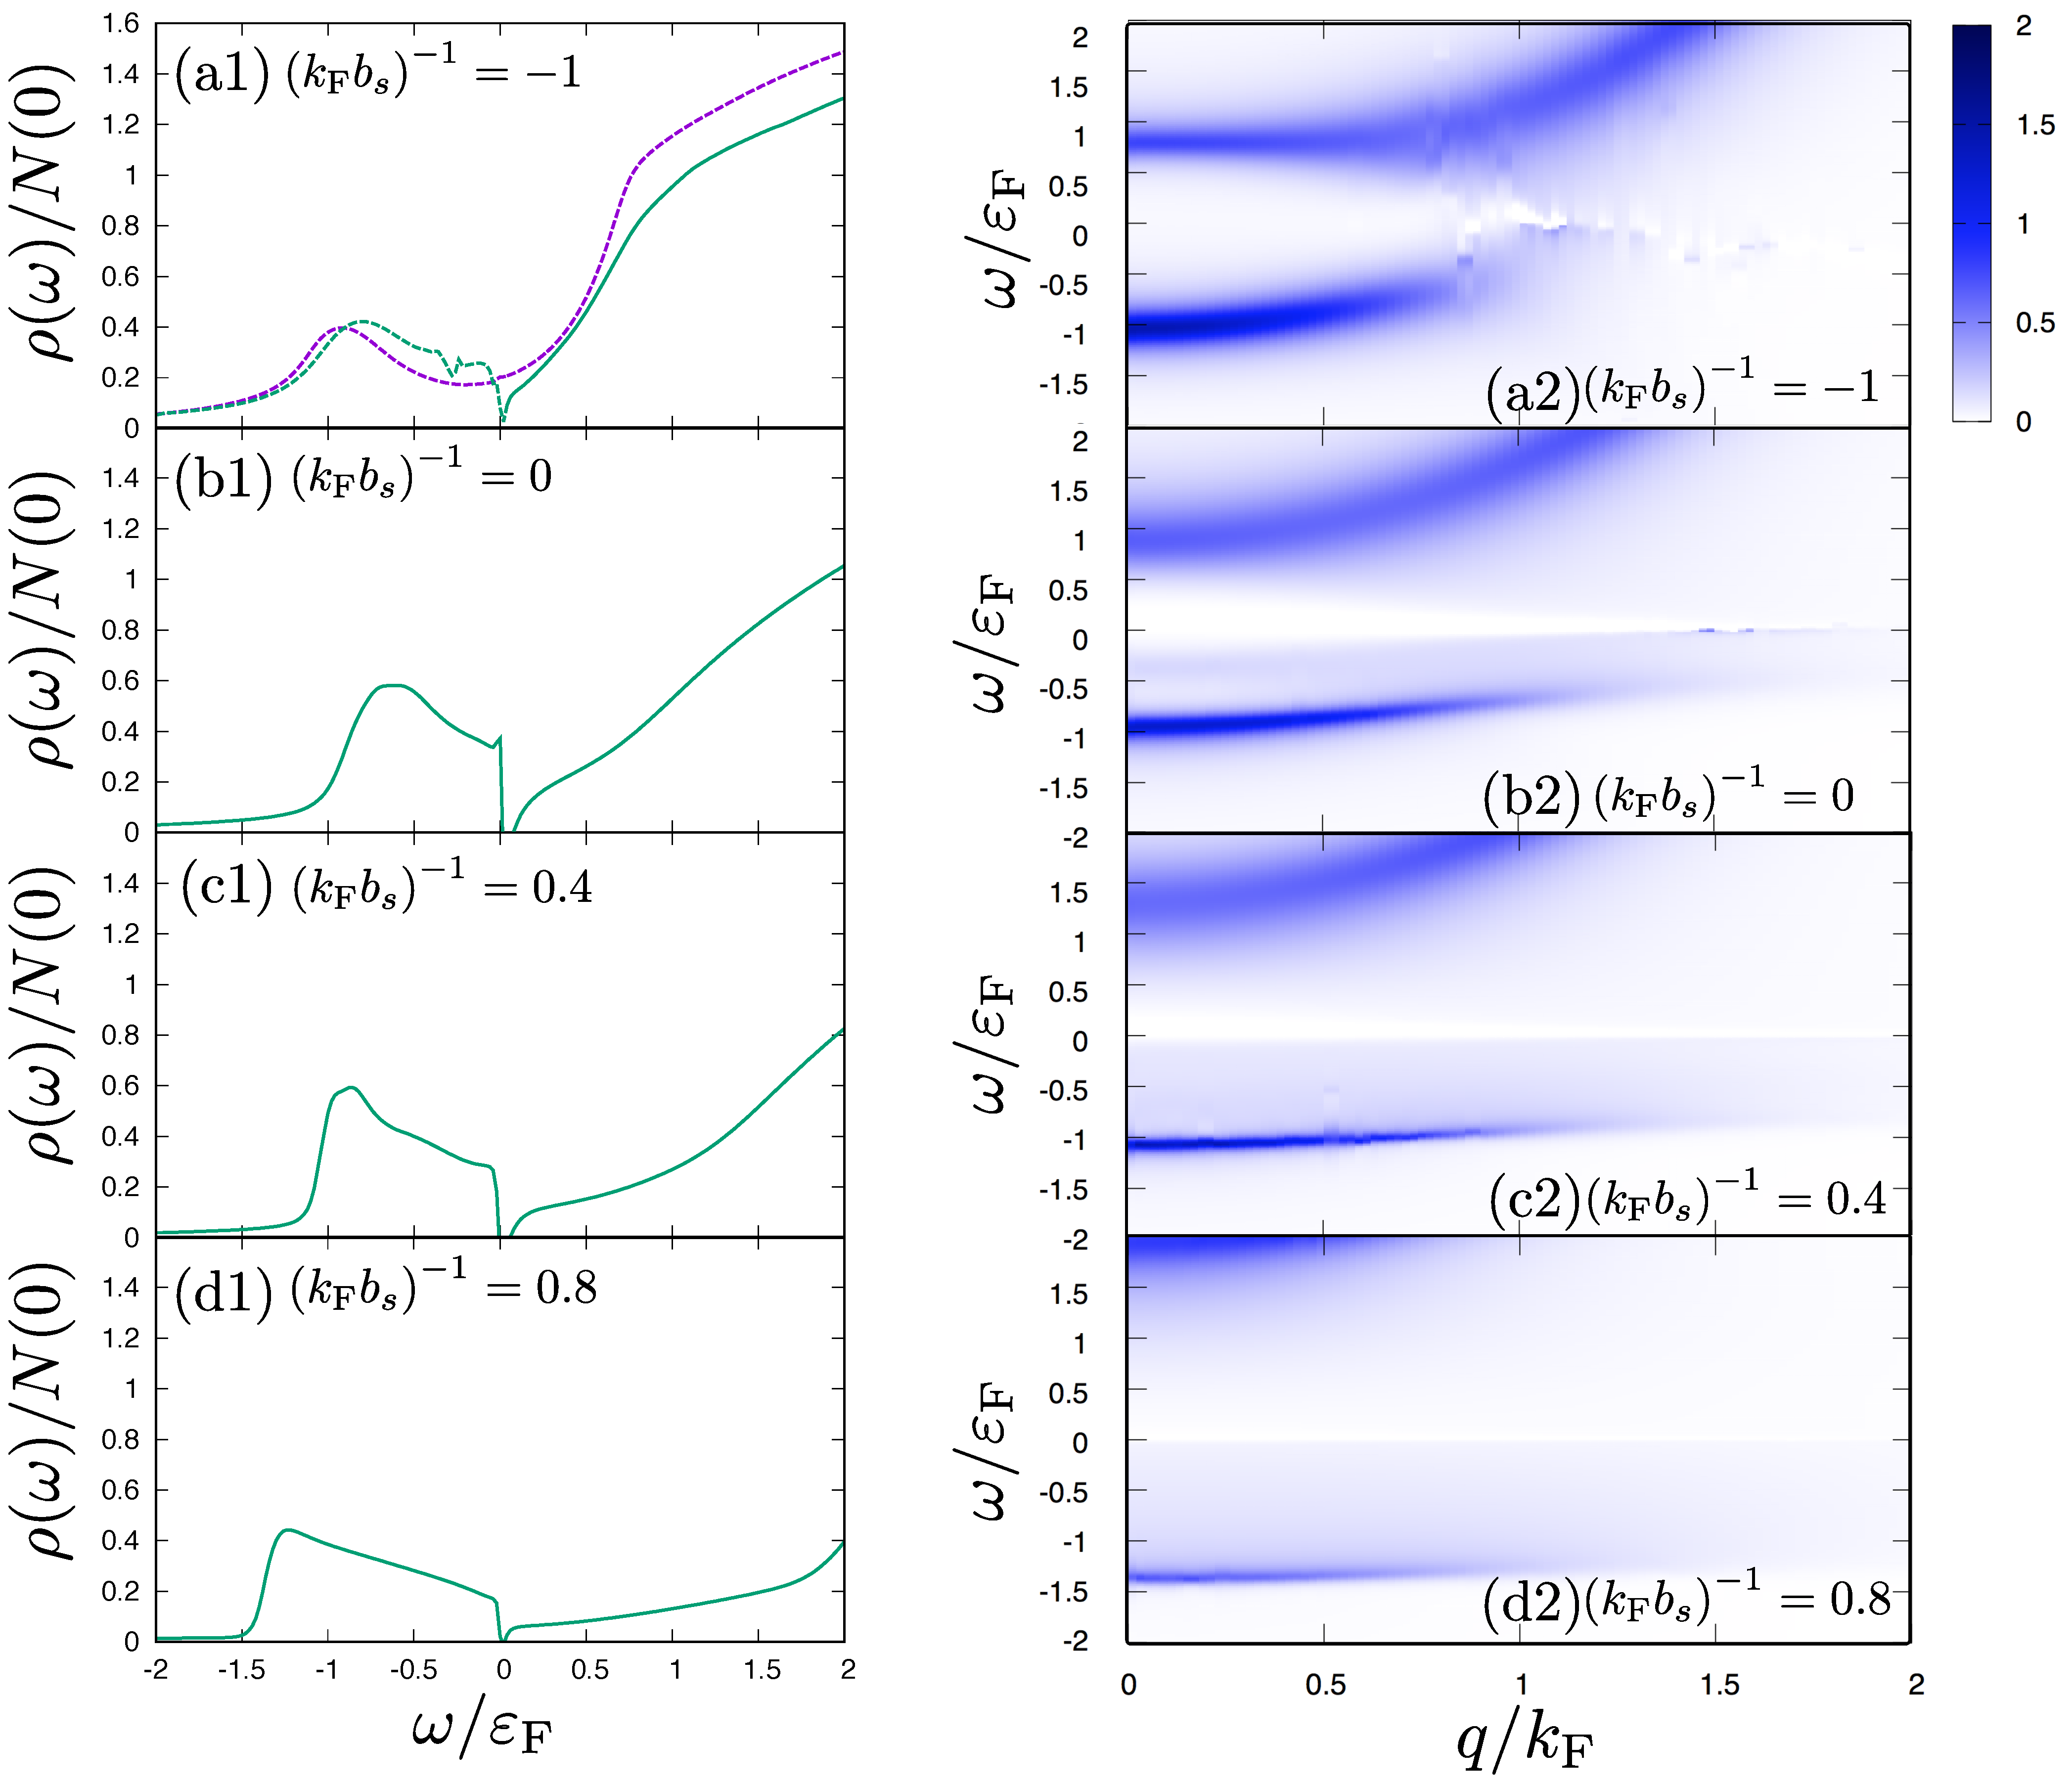
\includegraphics[width=130mm]{eps/tma-c1000-spe.eps}
\caption{図 \ref{fig:bcsl:imp:psgap} と同じだが $\overline{c}=1$ の場合。}
\label{fig:bcsl:imp:psgap2}
\end{figure}


式 (\ref{eq:bcsl:con:tctc0}), (\ref{eq:bcsl:con:cpcp0}) に見られるような $N'=(1-2\lc)N$ 粒子系への移行は擬ギャップ現象にも見られる。
擬ギャップ現象とは、超流動ゆらぎによって非凝縮のクーパー対が形成されることで、超流動転移温度以上においても超流動ギャップと同様に 1 粒子状態密度のフェルミ面近傍に窪み構造が現れる現象である。図 \ref{fig:bcsl:imp:psgap} に示すように不純物散乱強度が弱い場合のユニタリ極限の 1 粒子状態密度には擬ギャップが見られるが、これは、不純物がない場合の擬ギャップ構造とほとんど同じである(不純物がない場合の結果と完全に一致しないのは、図 \ref{fig:bcsl:imp:ndosc0500} の常流動状態における状態密度から、$\bskfi=-1$ の段階で自由粒子の底が $\omega+\mu=0$ から立ち上がらなくなっていることから、すでに多少の不純物準位の影響を受けているためであると考えられる)。ここから不純物散乱強度を強くしていくと、最終的には $N'=(1-2\lc)N$ 粒子系のユニタリ極限における(擬ギャップ構造のある) 1 粒子状態密度に帰着することがわかる。図 \ref{fig:bcsl:imp:psgap} の右側に示すように、スペクトル強度 $A_{\bp}(\omega)$ も (a)$\to$ (d) を見ると、$N$ 粒子系の擬ギャップ構造から、$N'=(1-2\lc)N<N $ 粒子系の擬ギャップ構造に漸近する様子が見て取れる。

これに対し、$\bskfi\gg1$ で、全原子が不純物に束縛されてしまう $\lc=0.5$ の場合は、図 \ref{fig:bcsl:imp:psgap1} に示すように不純物散乱の効果が強くなるにつれ、擬ギャップ構造は消失するが、(d1) の状態密度は単純な不純物を有する自由フェルミ気体の状態密度とは異なっており、状態密度の詳細な構造には、超流動揺らぎの影響があることがわかる。これは $\lc=1$ の場合にも見られる効果である(図 \ref{fig:bcsl:imp:psgap2})。ただし、これら後者 2 つの場合、$\bskfi=0.8$ での状態密度の構造の詳細が超流動揺らぎのどういう性質を反映したものであるか、については今後の研究課題である。


